\documentclass[11pt]{article}
\usepackage[a4paper]{geometry}
\usepackage[pdftex]{hyperref}
\usepackage[german]{babel}
\usepackage[utf8]{inputenc}
\usepackage{csquotes}
\usepackage{amssymb}
\usepackage{graphicx}
\usepackage{multicol}
\usepackage{amsmath}
\usepackage{fancyhdr}

\geometry{
  headheight=14pt,
  left=1cm,
  right=1cm,
  bottom=1cm,
  top=1cm
}

\setlength{\marginparsep}{1 cm}
\setlength{\topmargin}{-0.6in}
\setlength{\textheight}{9.5in}
\pagestyle{fancy}


% German-style quotation marks %
\MakeOuterQuote{"}

% Typesetting des Differentialoperators
\providecommand\d{}
\renewcommand{\d}[1]{\:\mathrm{d}{#1}} 

\fancypagestyle{firstpage}{%
  \lhead{\bf Name:}
  \rhead{\bf Anzahl zusätzlicher Blätter:\space\space\space\space\space}
  \cfoot{\textbf{(bitte wenden)}}
}

\begin{document}

\thispagestyle{firstpage}

\begin{center}
{\bf {\large Probeklausur Analysis (3IT18-1, 3MI18-1) - 27.02.2019}}
\end{center}

\begin{center}
\textbf {Der Rechengang muss eindeutig und vollständig ersichtlich sein!}

Diese Klausur bitte mit zusätzlich beschriebenen Blättern zusammenheften.
\end{center}

\textbf{Hilfsmittel}: Kein Taschenrechner, ein handbeschriebenes A4-Blatt.

\textbf{Erreichte Punktzahl}: $($\space\space\space\space\space + \space\space\space\space\space)$/47$ \space\space\space\space\space \textbf{Note}:

\section*{Klausuraufgaben}

\begin{enumerate}

\item Gegeben sei die Funktion $f(x) = \ln(2x-2)$.

\begin{enumerate}
\item (4P) Die Funktion $f$ ensteht aus der Funktion $g(x) = \ln(x)$ durch Verschiebung und Skalierung. Um wie viel und entlang welcher Achse wird verschoben und skaliert?
\item (3P) Skizzieren Sie die Funktion $f$! Tragen Sie den Wert von einem Punkt ein, durch den die Funktion verläuft (z.B. Nullstelle).
\item (3P) Welche Art von Monotonie hat diese Funktion? Was ist der Unterschied zwischen monoton steigend und streng monoton steigend?
\end {enumerate}

\begin{center}
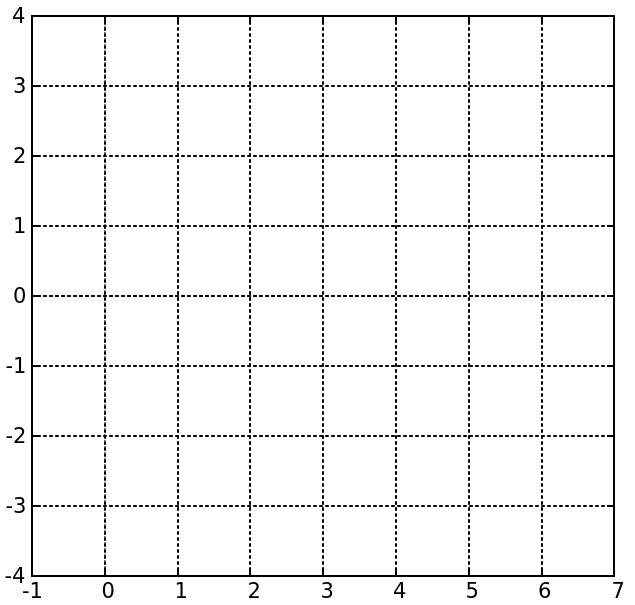
\includegraphics[width=0.5\textwidth]{grid_probe.png}
\end{center}

\item Eine Funktion $f(x)$ heißt achsensymmetrisch bzgl. der vertikalen Achse $x=k, k\in\mathbb{R}$, falls die folgende Bedingung erfüllt ist:

$$f(k-x) = f(k+x)$$

\begin{enumerate}

\item (4P) Untersuchen Sie anhand dieser Bedingung, ob $f(x) = x^2+9-6x$ symmetrisch ist bzgl. $x=3$!

\item  (3P) Es soll untersucht werden, zu welcher Achse $x=k$ die Funktion $f(x) = x^2+4x+4$ achsensymmetrisch ist. Die Auswertung der Bedingung ergab:

$$k^2-2kx+4k+x^2-4x+4 = k^2 + 2kx + 4k + x^2 + 4x +4$$

Welchen Wert hat k? (Hinweis: Zusammenfassen nach Potenzen von x, Koeffizientenvergleich)

\end{enumerate}

\item Die Ableitung einer Funktion $f(x)$ wird definiert über den Differenzialquotienten:

$$f'(x) = \lim\limits_{\epsilon\to 0} \frac{f(x+\epsilon)-f(x)}{\epsilon}$$

\begin{enumerate}
\item (2P) Schreiben Sie für $f(x)=\sin(2x)$ den Differenzialquotienten auf (ohne den Grenzwert zu berechnen).
\item (4P) Berechnen Sie seinen Wert für $f(x)=x^2+2$, d.h. führen Sie die Grenzwertbildung aus!

(Hinweis: Ausmultiplizieren, kürzen).
\end{enumerate}

\item Es soll das Integral der Funktion $f(x) = \frac{x^2+2}{x^3-4x}$ ermittelt werden. Die Partialbruchzerlegung ergab:

$$f(x) = \frac{x^2+2}{(x-2)\cdot x\cdot (x+2)} = \frac{A_1}{x-2} + \frac{A_2}{x} + \frac{A_3}{x+2}$$

Mit den Konstanten $A_1$ = $\frac{3}{4}$, $A_2=-\frac{1}{2}$.

\begin{enumerate}
\item (3P) Ermitteln Sie noch den Wert für $A_3$!
\item (2P) Berechnen Sie nun das unbestimmte Integral $\int f(x) \d x$!
\item (4P) Was wird graphisch durch das sogenannte "bestimmte Integral" berechnet? Was versteht man unter dem sogenannten "gerichteten Flächeninhalt"?
\end{enumerate}

\item Betrachtet werden soll die Differentialgleichung (DGL):

$$\frac{xy'}{y} = \sin(x)$$

\begin{enumerate}
\item (6P) Klassifizieren Sie diese DGL bezüglich Ordnung, Homogenität, Linearität. (Begründung!)
\item (3P) Sie kann mittels der Methode "Trennung der Variablen" gelöst werden. Geben Sie die beiden Integrale an, die dabei zu lösen sind!
\item (4P) Eines der beiden Integrale ist schwer zu lösen. Daher soll die Lösung genähert werden für kleine Werte $|x|$, indem der Term $\sin(x)$ in der DGL ersetzt wird durch seine Taylorentwicklung 3. Grades um die Stelle $x_0=0$. Geben Sie die dadurch entstehende DGL an!
\item (2P) Finden Sie die allgemeine Lösung der genäherten DGL!
\end{enumerate}

\end{enumerate}

\section*{Zusatzaufgabe (2P)}

Die Fakultät $a_z = (z-1)!$ einer natürlichen Zahl  $z$ ist charakterisiert durch die rekursive Eigenschaft $a_{z+1} = z\cdot a_z$. Für nichtganzzahlige Werte $z$ wird sie erweitert mittels der sogennanten Gamma-Funktion, diese ist definiert als $\Gamma(z) = \int\limits_0^\infty x^{z-1} e^{-x} \d x$. Zeigen Sie mittels partieller Integration, dass auch die Gammafunktion diese rekursive Eigenschaft erfüllt, d.h. dass $\Gamma(z+1) = z \cdot \Gamma(z)$ gilt!

\section*{Formeln}

Sie benötigen möglicherweise folgende Formeln:
\begin{itemize}
  \item Taylorentwicklung an Stelle $x_0=0$ lautet $f(x) = f(0) + f'(0)x + \frac{1}{2}f''(0)x^2+\frac{1}{6}f'''(0)x^3+...$
  \item Partielle Integration: $\int f(x)g(x)\d x = F(x)g(x)-\int F(x)g'(x)\d x$, wobei $F$ eine Stammfunktion von $f$ ist.
\end{itemize}

\newpage

\begin{center}
{\bf {\large Musterlösung}}
\end{center}

\begin{center}
\textbf{Jeder Anführungspunkt entspricht einem erteilten Bewertungspunkt.}
\end{center}

Pro Aufgabe gibt es einen Punkt Abzug, falls formal inkorrekte Schreibweisen verwendet werden (maximal 5 Punkte Abzug). Beispiel: 
$$f(x)=\sin(x), f'(x)=\sin(x)=0$$

Mit dem letzten Gleichheitszeichen ist eigentlich gemeint, dass $f'(0)$  berechnet wurde.

\begin{enumerate}

% Task 1
\item
\begin{enumerate}
\item $f(x) = \ln(2x-2) = \ln(2(x-1))$
\begin{itemize}
\item Verschiebung entlang x-Achse
\item 1 Einheit nach rechts
\item Skalierung (Stauchung) entlang x-Achse
\item mit dem (Skalierungs-)Faktor 2
\end{itemize}

\item Der Graph muss aussehen wie eine Logarithmusfunktion, die wie in $(a)$ beschrieben verschoben ist:
\begin{itemize}
\item Graph nähert sich der Vertikalen $x=1$, ohne sie zu schneiden
\item Graph ist monoton steigend mit Biegung im Uhrzeigersinn
\item Es wurden ein Punkt mit den korrekten Koordinaten eingezeichnet, z.B. $f(1.5) = \ln(2*1.5-2) = \ln(1) = 0$.
\end{itemize}

\item 
\begin{itemize}
\item Graph ist monoton steigend (genauer: streng monoton steigend)
\item streng monoton steigend heißt immer ansteigend
\item monoton steigend heißt Stagnation ist möglich
\end{itemize}

\end{enumerate}

% Task 2
\item
\begin{enumerate}

\item 
\begin{itemize}
\item $k=3$
\item $f(3-x) = (3-x)^2+9-6(3-x) = 9+x^2-6x+9-18+6x$
\item $f(3+x) = (3+x)^2+9-6(3+x) = 9+x^2+6x+9-18-6x$
\item Terme sind paarweise identisch, also achsensymmetrisch bzgl. $x=3$
\end{itemize}

\item 
\begin{itemize}
\item Identische Terme heben sich auf: $-2kx-4x=2kx+4x$
\item Umstellen: $-4kx = 8x$
\item Auflösen: $-4k=8$, also $k=-2$.
\end{itemize}

\end{enumerate}


% Task 3

\item
\begin{enumerate}

\item
\begin{itemize}
\item Das Argument $2x$ wurde korrekt eingesetzt, also $\sin(2(x+\epsilon))$, \textbf{nicht} $\sin(2x+\epsilon)$
\item $f'(x) = \lim\limits_{\epsilon\to 0} \frac{\sin(2(x+\epsilon)) - \sin(2x)}{\epsilon}$
\end{itemize}

\item 
\begin{itemize}
\item $f'(x) = \lim\limits_{\epsilon \to 0} \frac{(x+\epsilon)^2+2-(x^2+2)}{\epsilon}$
\item $\implies f'(x) = \lim\limits_{\epsilon \to 0} \frac{\epsilon^2+2x\epsilon}{\epsilon}$
\item $\implies f'(x) =\lim\limits_{\epsilon \to 0} \epsilon+2x$
\item $\implies f'(x) = 2x$
\end{itemize}

\end{enumerate}

\newpage

% Task 4

\item
\begin{enumerate}

\item
\begin{itemize}
\item $A_3 = \frac{(-2)^2+2}{(-2-2)\cdot(-2)}$
\item $A_3 = \frac{6}{8}$
\item $A_3 = \frac{3}{4}$ (Kürzen!)
\end{itemize}

\item 
\begin{itemize}
\item Es wurde der Betrag im Logarithmus verwendet.
\item $\int f(x)\d x = \frac{3}{4} \ln(|x-2|) - \frac{1}{2} \ln(|x|) + \frac{3}{4}\ln(|x+2|)$
\end{itemize}

\item 
\begin{itemize}
\item Es wird ein Flächeninhalt berechnet.
\item Und zwar der zwischen Graphen und x-Achse.
\item Oberhalb der x-Achse positiv gewertet
\item Unterhalb der x-Achse negativ gewertet
\end{itemize}

\end{enumerate}


% Task 5

\item
\begin{enumerate}

\item $xy'-\sin(x)y = 0$
\begin{itemize}
\item Ordnung 1
\item Weil $y'$ höchste Ableitung
\item Homogen
\item Weil $x(ty)'-\sin(x)(ty) = t^1(xy'-\sin(x)y)$
\item Linear
\item Weil Grad der Homogenität gleich 1
\end{itemize}

\item 
\begin{itemize}
\item $x \frac{\d y}{\d x} = \sin(x)y$ (Ersetzen von $y'$ durch $\frac{\d y}{\d x}$)
\item $\implies \frac{dy}{y} = \frac{\sin(x)}{x}$
\item $\implies \int\frac{dy}{y} = \int\frac{\sin(x)}{x}$
\end{itemize}

\item Betrachte $g(x)=\sin(x)$
\begin{itemize}
\item $f'(x) = \cos(x), f''(x) = -\sin(x), f'''(x) = -\cos(x)$
\item $f(0) = 0, f'(0) = 1, f''(0) = 0, f'''(0) = -1$
\item $\sin(x) \approx x -\frac{x^3}{6}$
\item Also genäherte DGL ist $xy'=y(x-\frac{1}{6}x^3)$
\end{itemize}

\item Näherung für $\sin(x)$ aus Aufgabe $(c)$ einsetzen in Ergebnis von Aufgabe $(b)$. Da abhängig von vorigen 2 Teilaufgaben, nur wenige Punkte:
\begin{itemize}
\item $\int\frac{dy}{y} = \int\frac{x-\frac{1}{6}x^3}{x}$
\item $\implies y(x) = \pm e^C e^{x-\frac{1}{18}x^3}$
\end{itemize}

\end{enumerate}

\end{enumerate}

\subsection*{Zusatzaufgabe}

\begin{itemize}
\item $\Gamma(z+1) = \int_0^\infty x^z e^{-x} \d x$
\item $= \underbrace{\big[ -x^z e^{-x}\big]_{0}^{\infty}}_{=0-0} + z \underbrace{\int_0^\infty x^{z-1}e^{-x}\d x}_{\Gamma(z)} = z\cdot\Gamma(z)$
\end{itemize}


\end{document}
